\documentclass[14pt,twoside,a4paper]{extarticle}
\usepackage[margin=2.5cm]{geometry}
\usepackage{graphicx} \graphicspath{{figure/}}
\usepackage{float} \usepackage{amsmath}
\usepackage[backend=biber]{biblatex}
\addbibresource{bibliografia.bib}

\title{Path planning locale per robot mobili \\ basato su potenziali artificiali alternati}
\author{}
\date{} 

\begin{document}

\maketitle \newpage %frontespizio
\tableofcontents \newpage %sommario

\section{Introduzione}
È innegabile che in questi anni si stia assistendo ad un aumento vertiginoso di sviluppo ed uso della robotica. È importante però evidenziare una distinzione tra due concetti apparentemente simili, ma per certi versi opposti, che caratterizzano due macro-categorie della robotica: automazione e autonomia. Il primo riguarda quei robot, tipicamente industriali, che operano in ambienti noti a priori ed eseguono in loop un compito predefinito; automatizzare, perciò, vuol dire sostituire l'essere umano in compiti ripetitivi e solitamente privi di eventi inaspettati. L'autonomia, invece, ben più complessa da realizzare, é caratteristica di quei sistemi che hanno un certo grado di inconsapevolezza sul proprio futuro e l'ambiente circostante.  Il robot, quindi, é definito autonomo se é un agente intelligente situato nello spazio fisico, dove un agente intelligente si definisce come un'entità che \textbf{osserva} l'ambiente e prende delle \textbf{azioni} per massimizzare il raggiungimento del suo \textbf{obiettivo}\cite{murphy}. Nel caso specifico di questa tesi, l'ambiente del robot autonomo é lo spazio bidimensionale (una superficie), e il suo obiettivo é un punto in questo spazio. Massimizzare il raggiungimento di questo punto vuol dire arrivarci nel minor tempo possibile, senza collidere con eventuali ostacoli. Quindi, il robot autonomo deve compiere una serie di azioni, non note a priori e definite da un algoritmo di pianificazione che si basa sui dati osservati dai sensori, per spostare la sua traiettoria, al fine di evitare collisioni e raggiungere comunque l'obiettivo. La tipica architettura di navigazione di un robot autonomo é data perciò da quattro moduli, detti anche primitive: 
\begin{description}
\item[Percezione] Prende in input le informazioni derivanti dai sensori, le processa e le restituisce
\item[Localizzazione e Mapping] Con le informazioni sensoriali, il robot costruisce una rappresentazione del proprio intorno basandosi sulla propria posizione e ciò che osserva. Il risultato globale, dopo aver fatto varie osservazioni di intorni diversi, sarà una mappa dell'ambiente, rispetto alla quale il robot può localizzarsi. (Per scopi esemplificativi, questo modulo verrà tralasciato nell'algoritmo di questa tesi, e si userà descrivere la posizione del robot con coordinate assolute e non rispetto ad una mappa.)
\item[Pianificazione] In base alle informazioni sensoriali e cognitive in possesso, produce in output delle decisioni ad un livello di astrazione alto. Nel caso del motion planning, la direttiva da produrre é il percorso da seguire.
\item[Azione] Prende in input le direttive del modulo di pianificazione e produce dei comandi a basso livello per gli attuatori del robot.
\end{description}
L'architettura utilizzata in questa tesi é la cosiddetta gerarchica: le quattro primitive vengono eseguite in ordine e in loop. È particolarmente indicata per problemi in cui l'obiettivo finale é ben definito a priori. In altre parole, non vi é nessun meccanismo di apprendimento nel robot, ma semplicemente pianificazione deterministica orientata al goal. In figura é visivamente sintetizzato quanto appena detto.

\begin{figure}[H]
\caption{Architettura di navigazione\cite{mac2016}}
\centering
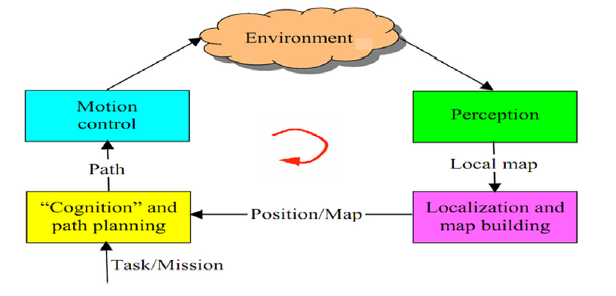
\includegraphics[scale=0.6]{architetturaNavigazione.png}
\end{figure}

In questa tesi viene affrontato un problema che rientra nel terzo modulo: il path planning, un problema di grande importanza e argomento di molta ricerca. Una sua rapida formulazione potrebbe essere la seguente: data la posizione iniziale (del robot) A e una posizione finale B, imposta da chi fa uso del robot, il path planning consiste nel calcolare un percorso fisicamente realizzabile e ottimale per arrivare da A a B.\\ 
All'interno dei metodi esistenti (e non), ci sono due importanti distinzioni da fare: sulla formulazione del problema e sulla soluzione al problema.
\begin{description}
\item[La prima] é tra online e offline path planning, o anche locale e globale. Il path planning globale riguarda quelle situazioni in cui l'ambiente considerato é interamente noto a priori, per cui é possibile calcolare il percorso da seguire ancor prima che il robot inizi a muoversi; quello locale é inerente ai casi in cui il robot debba fare i conti lungo il suo percorso con eventi inaspettati, quali ostacoli dinamici,per cui é necessario reagire localmente, aggiornando ripetutamente le informazioni derivanti dai sensori e aggiustando la traiettoria al fine di evitare l'ostacolo e poter raggiungere in tempi ottimali l'obiettivo.
\item[La seconda] distinzione é tra soluzioni basate su tecniche di intelligenza artificiale - la cui trattazione esula dagli scopi di questa tesi - e soluzioni classiche. Quest'ultime possono ulteriormente essere suddivise in \cite{siciliano}:
\begin{itemize}
\item{Subgoal (o anche roadmap)}\\ 

\item{Decomposizione in celle}
\item{Sampling based} RRT ecc
\item{Potenziali artificiali} Li descrivo meglio avanti
\end{itemize}
\end{description}

Nota : Ancora da fare breve descrizione dei metodi

La totalità dei metodi appena descritti risolvono adeguatamente il problema del path planning globale.\cite{dalfonso} 

\begin{figure}[H]
\caption{Classificazione algoritmi di path planning\cite{mac2016}}
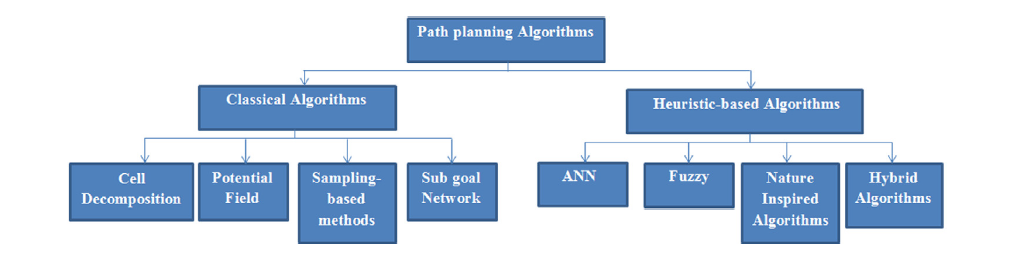
\includegraphics[width=\textwidth]{algoritmiPP.png}
\end{figure}

Come da titolo, questa tesi ha come obiettivo specifico quello di esporre un lavoro di progettazione, implementazione e simulazione di un algoritmo di path planning \textbf{locale} basato su \textbf{potenziali artificiali discretizzati e alternati}. 

\section{Potenziali artificiali}
Illustrazione metodo classico\\
Illustrazione problema minimi locali\\
Accenno al metodo dei potenziali artificiali evolutivi\\
Accenno al metodo limit cycle\\
Illustrazione potenziale vorticoso (potenziale e antigradiente)

\section{Formalizzazione del problema\cite{dalfonso}}
Chiamerò \( r(t) = [x_r(t),y_r(t),\theta_r(t)]^T\) la posizione del robot nell'istante attuale t e \( O_i(t) = [x_(O,i)(t),y_(O,i)(t)]^T, i = 1...N\) la posizione degli N ostacoli che, per scopi esemplificativi, saranno di forma circolare e con raggio \(R_i\). Esisterà inoltre un punto \(G = [G_x, G_y]\). Il problema consiste nel voler raggiungere il punto \(G\) dalla posizione iniziale \(r(0)\), tenendo conto degli \(N\) ostacoli in movimento. Il robot é dotato di un raggio di visione di \(R_v\) unità di lunghezza, entro il quale é capace di rilevare un ostacolo. Inoltre, si presuppone che valga la seguente condizione
\[\begin{Vmatrix}\begin{bmatrix} x_r(t)\\ y_r(t) \end{bmatrix} - O_j(t)\end{Vmatrix} \leq R_v \], ovvero \( R_i \leq R_v, \forall i\). Ciò vuol dire che nel momento in cui il robot incontra un ostacolo, il centro di quest'ultimo é incluso in \(R_v\).

\section{Algoritmo di navigazione\cite{dalfonso}} 
La strategia é semplice: nella posizione iniziale, il robot sonda l'ambiente attorno a sé. Se non vi sono presenti ostacoli a impedirne l'avanzamento verso il goal, la traiettoria da seguire é quella imposta dal potenziale attrattivo; altrimenti, é necessario "switchare" dal potenziale attrattivo a quello vorticoso, al fine di aggirare l'ostacolo, per poi tornare a seguire la traiettoria. Perciò, la peculiarità di questo algoritmo é che in ogni istante il robot seguirà un solo potenziale alla volta, evitando così il problema dei minimi locali. Inoltre, le informazioni necessarie a pianificare lo switch non richiedono informazioni globali, ma solo quelle riguardanti l'ostacolo da aggirare.

\subsection{Interazione con l'ambiente}
Come viene costruito l'ambiente (grid)\\
\subsubsection{Percezione}
Come vengono percepiti gli ostacoli e le loro velocità\\
Come viene percepita la propria posizione (accenno localizzazione)\\
\subsubsection{Azione}
Modello cinematico\\
Legge di controllo\\
Come faccio muovere il robot nella grid

\subsection{Pianificazione}
Data la struttura intrinseca della strategia di navigazione che si basa su un meccanismo di switching tra due stati, per definizione mutuamente esclusivi, un modo per modellare visivamente l'algoritmo é lo statechart diagram in figura. Il robot può trovarsi o nello stato corrispondente al potenziale attrattivo, oppure in quello corrispondente al potenziale vorticoso. In quest'ultimo esistono altri due sottostati, la cui natura verrà spiegata meglio in seguito.
	
\begin{figure}[H]
\caption{Statechart Diagram} \label{state}
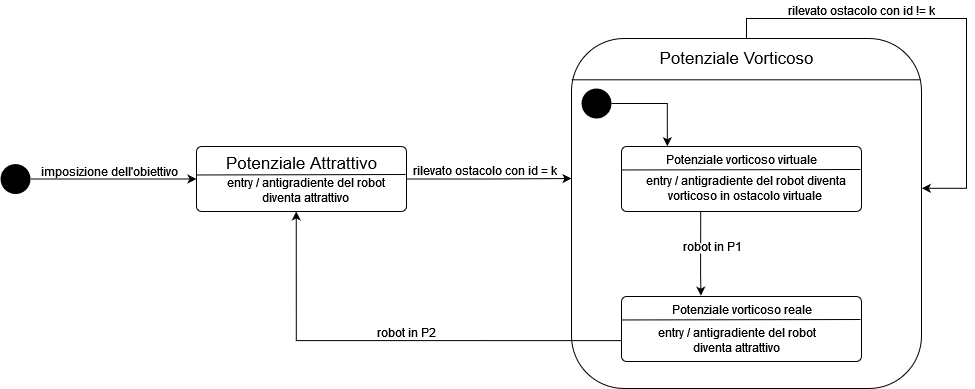
\includegraphics[width=\textwidth]{stateDiagram.png}
\end{figure}
	
Note	: caso 1 sto seguendo il potenziale attrattivo e passo al vorticoso (calcolo verso, calcolo xOmega e yOmega, calcolo P1 e P2, calcolo due potenziali con relativi c), caso 2 sto seguendo il vorticoso e passo all'attrattivo (reimposto attrattivo)
	
\begin{figure}[H]
\caption{Flowchart Diagram} \label{flow}
\centering
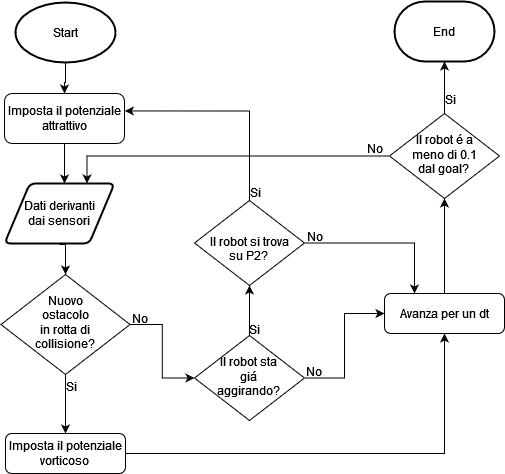
\includegraphics[width=0.8\textwidth]{flowchartDiagram.png}
\end{figure}

\section{Testing e risultati}
Parametri utilizzati\\
Un ostacolo fermo e in movimento\\
Minimi locali e confronto con potenziali artificiali classici\\
Tre in movimento\\

\section{Simulazione con Gazebo (o Turtlesim)}

\section{Applicazioni e sviluppi futuri}

\newpage
\listoffigures
\printbibliography

\end{document}
